\section{Introduction}

A significant step towards understanding today's advancements in Reinforcement Learning (RL) is by first understanding the fundamental theory of Markov Decision Processes (MDP) for modeling decision making problems and the ``exact'' model-based algorithms that optimally solve these problems. However, these approaches are limited by their requirement for complete knowledge of the environment (model). A major breakthrough in RL was thus the development of the Q-learning algorithm, the first model-free learning algorithm with guaranteed convergence to the optimal policy.

In this report I present my course project implementing these algorithms and analyzing their ability to maximize earnings on a simplified, ``toy'' version of poker. I will start by first establishing the rules of this simplified game, the opponents designed as part of the environment, my model representation and how I implemented all of them in Python. With the problem formulation being established, I will then continue with how I applied Policy Iteration (model-based) and Q-learning (model-free) algorithms to this problem, reporting key observations, and most importantly, analyzing their behavior due to the nature of this game and what theory predicts.

\section{Environment}

\subsection{Simplified game rules}

Both ``exact'' algorithms are limited in solving problems with a relatively small number of states and actions. As poker is characterized by numerous parameters (number of players, position/order of players, legal actions, bidding round number, betting chip/token allowance, hidden and public cards, winning card combinations), the state-space quickly has a large number of states. To alleviate this issue for the purposes of this project, a simplified version of the most popular poker variant, Texas hold'em was used. Since Texas hold'em is a well-known game and its rules are also summarized in the project description, I will only provide a quick summary of its rules here, with emphasis on the unique deviations assumed here.

First of all, a dumped-down version of heads-up limit Texas hold'em is used as a basis, thus only 2 players participate. Both players start with a card in hand (not the normal of 2 cards) and with betting the same mandatory amount of 0.5 tokens (namely no small/big ``blind'' difference). 

The game continues with a bidding round. Since this is a limit variant, either 1 (actions ``bet'' or ''raise'') or 0 (actions ``check'' or ``fold'') tokens can be placed by a player per turn of action, with a maximum of 2 tokens placed in total by each player per round. If a player folds, the other player is an instant winner and is rewarded with the full amount of tokens bet so far. Otherwise, 2 cards are further drawn and are publicly revealed, and a second bidding round, similar to the first one, begins. Unlike the real game, the order (position) of players in which they are required to take action remains the same for both rounds. For simplicity, no further rounds and card draws take place. Table \ref{table:actions}(a) summarizes the legal order of actions in all game states.

Assuming no player has folded until the end of round two, the winner is then decided by comparing their ``hand strength''. To reduce the number of possible combinations, only cards with rank `T', `J', `Q', `K', `A' (in ascending order) are available in deck (20 cards in total, 4 suits per rank). This simplification leaves only three winning combinations of hand and public cards: 1) 3 cards of the same kind (rank), 2) a pair of same kind, 3) no pairs. The rank of the pair or hand is used as a tie-breaker in rules (2) and (3). If all tie-breakers fail, the result is a tie and the tokens placed by both players are returned to them.

\begin{table}[htpb]
\centering
\resizebox{\linewidth}{!}{%
\subfloat[]{\begin{tabular}{ |c|c|c| }
\hline
position & opponent chip difference & legal actions\\
\hline
\hline
first & 0 & bet, check \\
\hline
first & 1 & bet, fold \\
\hline
second & 0 & check, raise \\
\hline
second & 1 & bet, fold, raise \\
\hline
\end{tabular}}
\quad
\subfloat[]{\begin{tabular}{ |c|c|c|c| }
\hline
round & hand strength & Threshold action priority\\
\hline
\hline
1 & A, K & 1. raise, 2. bet \\
\hline
1 & J, Q & 1. check, 2. bet \\
\hline
1 & T & 1. check, 2. fold \\
\hline
2 & pair or better & 1. raise, 2. bet \\
\hline
2 & A, K, Q (no pair) & 1. check, 2. bet \\
\hline
2 & J, T (no pair) & 1. check, 2. fold \\
\hline
\end{tabular}}
}
\caption{(a) Legal actions of players according to their position and difference between opponent's and player's chips. (b) The actions a Threshold agent selects at any possible state. If both actions shown are legal, the one with higher priority (lower number) will be selected.}
\label{table:actions}
\end{table}

\subsection{Opponents as part of the environment}
\label{sec:opponents}

Two different types of ``static'' (non-adversarial) agents were created in this project. These opponents serve as both necessary components of the full state-space formulation required by Policy Iteration, and benchmarks for the performance of Q-learning.

The first opponent, hereafter called \textit{Random agent}, is a completely randomized agent. Each time an action is required by it, it randomly picks -with equal probability- one of the actions allowed according to the game's current phase. Since the Random agent disregards any other card and opponent information, its opponent cannot infer any meaningful information from its actions.

The second opponent, named \textit{Threshold agent}, is a completely deterministic agent, using only the strengths of its cards to determine its next action. Table \ref{table:actions}(b) summarizes the action this agent will perform at any possible step. In contrast to the Random agent, each and every action of the Threshold agent provides information on the range of possible ranks held in its hand. Therefore, its predictable nature can be used against it by any agent trained on it.

\subsection{MDP and state/action space representation}
\label{sec:state-space}

Before proceeding with the implementation and results of this work, careful formulation of the state-space representation is crucial. This representation should balance between two opposing ends: 1) be as complete as possible to capture all information required by the ``exact'' algorithms used here, 2) have the smallest size possible to reduce computational demands without sacrificing completeness. The state representation used in this project is fully characterized by six features. For a detailed depiction of all features, also discussing both their necessity and how their value range was optimized, please see Appendix Table \ref{table:state-space}.

Each state of the MDP is coupled with its legal actions only. Each state-action pair is then linked to one or more possible transitions. Each transition is in turn characterized by: 1) its conditional probability (given the state-action pair), 2) the next state, 3) the associated reward (which for a loss is negative), and 4) terminal status (as boolean). Note that in Texas Hold'em games, all intermediate states have 0 reward, and only terminal states may have non-zero values (and 0 only in case of ties).

\subsection{Implementation}

The entirety of this project was implemented in Python. All simulations and results reported here can be reproduced by running the Jupyter Notebook file \Verb|notebook.ipynb|.

In regards to the environment implementation of this simple poker variant, I adapted the corresponding object-oriented game structure of the \href{https://rlcard.org/}{rlcard} Python library. Although this library may have already contained a functional environment for a number of poker games, this project's unique game rules demanded novel implementation of almost all classes.

In summary, the \Verb|Card| class models each possible card of the game, while the \Verb|Dealer| is responsible for maintaining the deck and drawing cards. The \Verb|Judger| class contains the aforementioned rules of winning and is responsible for deciding the payoffs of each player (implemented as \Verb|Player| objects containing the state features known to each one). A \Verb|Round| object encapsulates all rules associated with player position, legal actions of currently active player, effects of selected actions, and round completion. The \Verb|Game| class is responsible for synchronizing all the aforementioned objects so that poker games can be executed as described.

As far as player types are concerned, they are modeled as agent classes. The two static agent models described in Section \ref{sec:opponents} are implemented by the \Verb|RandomAgent| and \Verb|ThresholdAgent| classes. Moreover, the agent classes trained using the Policy Iteration and Q-learning algorithms include the implementation of these algorithms and are named \Verb|PolicyIterationAgent| and \Verb|QLearningAgent| respectively. As a way for a human player to test the environment and play against a computer-controlled agent, the \Verb|HumanAgent| class is also included (see file \Verb|play.py| for an example script to try it out).

To run games, the \Verb|Env| class brings together the \Verb|Game| and opposing agent objects, is responsible for invoking the \Verb|Game| functions and extracting the complete current state representation. Finally, file \Verb|seeding.py| contains random seeding utility functions offered by rlcard, while a few generic utility functions are implemented in file \Verb|utils.py|.

\section{MDP-based solution: Policy Iteration algorithm}

Prior to experimenting with a true learning algorithm in this game, we first want to acquire a clear understanding of the environment. As already mentioned, modeling the environment (the combination of game rules and opponent behavior) as an MDP enables us to solve the problem optimally with dynamic programming methods such as Policy Iteration. Therefore, I start this section by highlighting my Python implementations of the MDP described in Section \ref{sec:state-space}, for both Random and Threshold opponents. Next, I rationalize my choice of hyperparameter configuration for Policy Iteration, I continue with reporting the results of this algorithm, and finally conclude with an analysis of the yielded optimal policies.

\subsection{MDP implementation}

As already mentioned, a state is fully characterized by six features. Since my primary goal was to enhance readability of my implementation and results, I sacrificed memory usage efficiency by selecting a descriptive state representation using Python's dictionaries over lists. In particular, a two-level nested dictionary structure was formed, with state being the first level key, action being the second level key, and each state-action pair containing a list of all possible transitions (which are as described in Section \ref{sec:state-space}). The syntax of state keys (following Table \ref{table:state-space}) is {\small \Verb|{{position}}_{{my_chips}}_{{opponent_chips}}_{{hand}}_{{public_cards}}_{{opponent_range}}|}, \\ while the action values in Tables \ref{table:actions} were directly used as action keys.

Since transition probabilities are entirely determined by 1) opponent action probabilities (opponent model), and 2) poker card probabilities (game rules), I needed to implement a way of calculating these odds for the unique poker variant of this project. Since the former is part of the game and irrespective of opponent models, I developed the function \Verb|get_transition_probabilities_for_cards()| in the Game class. This function returned a dictionary containing the odds of each card pairs (as ranks) being drawn in flop knowing our hand and our opponent's range (resulting file \Verb|win_probabilities.json|). Now given the public cards as well, this method also provides the odds of winning (file \\ \Verb|win_probabilities.json|) and losing (file \Verb|loss_probabilities.json|), with tie odds also being trivially calculated. Finally, resulting file \Verb|range_probabilities.json| includes the odds of the opponent having a certain card range given their current range and all other revealed cards.

In regards to opponent action probabilities, these of course differ between Random and Threshold agents based on their definition in Section \ref{sec:opponents}. To this end, their calculation in both corresponding classes is part of function \Verb|calculate_state_space()|. With this function I programmatically calculate all possible state-action-transition combinations. In the case of Random agent this function yielded 1000 non-terminal states and 2230 non-terminal state-action pairs (see file \Verb|random_agent_state_space.json|), whereas for Threshold Agent the state space was larger with 2075 non-terminal states and 4500 non-terminal state-action pairs (see file \texttt{threshold\_agent\_state\_space .json}). The reason behind this difference is due to inference of the Threshold opponent's possible range of hands based on its actions, whereas we cannot infer any information based on a Random opponent's actions (see last feature of Table \ref{table:state-space}).

\subsection{Algorithm implementation and hyperparameter configuration}

For the development of Policy Iteration agent, I adapted the example for the Frozen Lake environment provided in class. Most of the provided implementation remained unchanged, however since I decided to use dictionaries for the representation of state-action-transitions, I had to replace the functionality meant for tabular representations with an equivalent for dictionaries.

Policy Iteration offers a pair of hyperparameters: 1) the convergence error $\delta$, and 2) the discount factor $\gamma$. My chosen values for both hyperparameters was supported by the episodic nature of limit poker, since all games terminate after a very limited number of state transitions. Therefore, for convergence error I chose the default low value of $10^{-10}$ (since fast convergence is expected). Furthermore, I also defaulted $\gamma=1$. Choosing a lower value for $\gamma$ in poker is expected to motivate a more aggressive gameplay, trying to winning games as fast as possible by forcing opponents to fold. However, I did not go that route since 1) rewards are equally important regardless of how many steps a game lasted, and 2) longer lasting games may offer more opportunities for increased rewards, especially against simple opponents that have a high chance of choosing subpar actions.

\subsection{Results}

Having set the MDP and hyperparameters, we can now evaluate the performance of Policy Iteration both in terms of convergence to the optimal policy and of average payoffs per game.

First, as expected, convergence is rapidly achieved. Although speed of convergence depends on policy initialization which is random, most of the times only 3 iterations of policy evaluation and improvement are enough to reach the desired level of convergence (2-4 has been observed in numerous tries). Note that lowering $\gamma$ a bit had only a effect on the resulting optimal policies, nevertheless this small effect was towards the expected direction of more aggressive playstyle (more bets/raises as optimal policies). These results were consistent against both Random and Threshold opponents.

Concerning the average payoffs achieved by the generated optimal policy per opponent, I tested them against their intended opponent in $5\cdot10^6$ simulated games. Expectedly, the Random agent was proven to be the worst player, providing a much larger margin for earnings (mean: 0.8761 tokens, standard deviation: 2.127 tokens) when compared to the more `rational' Threshold agent (mean: 0.2251, std: 1.467). 

\subsection{Optimal policy analysis}

Interpreting the optimal policy generated by Policy iteration requires a firm understanding of the environment. Furthermore, proving its optimality is challenging due to the large state-space of this game. Nevertheless, in this section I present a brief interpretation of the policies generated for both opponents, and a few sanity checks to support that they are indeed optimal.

\subsubsection{Random opponent}

Inspecting the optimal policy for Random opponents (file \Verb|random_agent_optimal_policy.json|), most profits are made by abusing the odds of it randomly folding at any step of the game. This is especially obvious when being in the advantageous second position, since the policy of always raising has at least a 50\% chance of winning the game due to a random fold, and thus raising is always the optimal action (`fold' and `bet' are the only legal options of the Random agent, let alone any chances of winning due to superior hand in case of `bet').

Similarly, betting at the beginning of a round when playing first always grants you at least 1/3 chances of winning. Therefore, in 215 out of 230 such states the hand strength is enough to make betting is the optimal action, while the remaining 15 states are post-flop cases with very weak hands, where `check` is indeed optimal. The optimal policy is slightly more conservative (75 out of 300 such states where fold is better than bet) is in the last possible action of a game after a post-flop raise, since then the chances of winning are entirely based on hand strength. These are the only states where fold may be optimal.

Finally, as an extra sanity check, I pitted the Random and Threshold agents against each other in the same experimental setup ($5\cdot10^6$ games). Even though the Threshold agent is a more rational player and still beats the Random agent, the results (mean payoffs: 0.3093, std: 1.643) clearly shows that it is far from being the optimal policy.

\subsubsection{Threshold opponent}

Analyzing the optimal policy for Threshold opponents (file \texttt{threshold\_agent\_optimal\_policy .json}) is not so straightforward, since we can now ``read'' these opponents based on their actions, resulting in a larger state-space. Nevertheless, a few trends are also apparent here and are ultimately entirely based on card odds (even opponent actions), which in general results in a tighter playstyle when compared to the optimal policy for Random opponents. 

Seeing a few examples: 1) Despite the weak hand, raise is optimal for state \Verb|second_0.5_0_T_AK_JQT|, since the Threshold opponent also has a weak hand and will fold more times than call (will call only if it has a Q). 2) For state \Verb|second_0.5_0_T_AJ_Q|, check is optimal because a loss is guaranteed; the opponent will never fold with a Q, and T loses against Q anyway. 3) For state \Verb|first_0.5_0_A_KQ_AK|, check is the best action because there is no chance for a Threshold agent to fold here, and the best we can do is a tie (if it has A). 4) For state \Verb|first_0.5_0_A_KK_JQT|, our win is guaranteed and betting may also increase our reward (if the Threshold agent has a Q will call).

In conclusion, as we will see in the following sections (and in Tables \ref{table:random-results}-\ref{table:threshold-results}), Policy Iteration indeed yielded the best policy per opponent out of all policies shown in this project.

\section{Model-free solution: Q-learning algorithm}

Now that we have a much better understanding of the environment, we are ready to experiment with a true learning algorithm, Q-learning. Although this method still needs a finite state-action space to be defined, no MDP and prior knowledge of transitions are needed. Therefore, the opponent is initially unknown and Q-learning adapts its policy while playing against it. In the rest of this section, I start by shortly describing my implementation and hyperparameter configurations. Next, I present the experimental design and results to evaluate the performance of Q-learning, comparing both with the optimal policy from Policy Iteration and between different hyperparameter configurations.

\subsection{Implementation}

For the purposes of this project I chose to implement the Q-learning algorithm shown in the coursebook of Sutton, Barto, chapter 6.5. In order to be able to evaluate the testing (and not training) performance of the Q-learning agent, I made the activation of both the temporal difference control (update) and the $\epsilon$-greedy steps configurable. Furthermore, if multiple actions are tied with the maximum (over all actions) $Q$ value, I chose to implement random action selection, which I also applied for initialization, to prevent tie breaking/initialization effects on convergence.

\subsection{Hyperparameter configuration}

The implemented Q-learning algorithm has three hyperparameters: 1) the discount factor $\gamma$ (which I simply set to 1 for the same reasons I did for Policy Iteration), 2) the $\epsilon$ for $\epsilon$-greedy state-action exploration, and 3) the learning rate $\alpha$. To guarantee convergence in the limit, I set both $\epsilon$ and $\alpha$ using an exponential decay function over the number of training episodes (games) $t>0$, as $\epsilon = \epsilon_0 t^{\epsilon_d}$ and $\alpha = \alpha_0 t^{\alpha_d}$, where $\epsilon_0$, $\alpha_0$ are the initial values (set for $t=0$ as well), and $\epsilon_d$, $\alpha_d$ are the corresponding decay rates. 

\subsection{Results}

To exhibit the effects of hyperparameter values on Q-learning performance, I set up the following experimental design: using a set of values for $\epsilon_0$, $\alpha_0$, $\epsilon_d$ and $\alpha_d$ as a basis, I trained the Q-learning agent with $3\cdot10^6$ games (as training set) versus its opponent. Subsequently, I used the pretrained agent against the same opponent in another $10^6$ games (as test set). I then repeated this process 5 times to measure the average testing performance of the Q-learning agent out of $5\cdot10^6$ games in total. Finally, I repeated the same process with 4 more sets of hyperparameter values, every time changing only a single parameter.

In the following subsections I present the results of these experiments against the Random and Threshold agents.

\begin{figure}[htpb]
\renewcommand*\thesubfigure{\alph{subfigure}}
\centering
	\subfloat[]{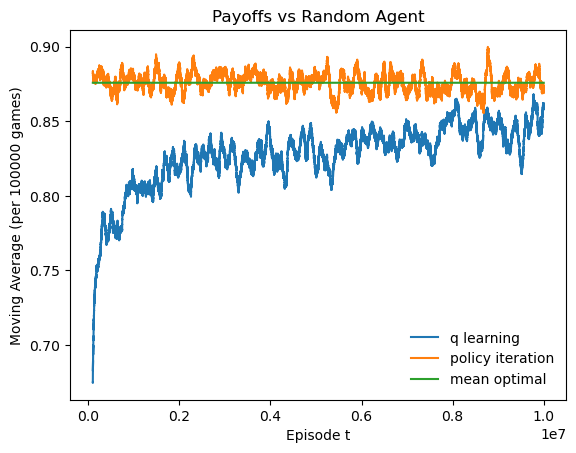
\includegraphics[width=0.33\textwidth, angle =0, trim = 0mm 0mm 0mm 0mm,clip=true]{figures/moving_averages_random}}
	\subfloat[]{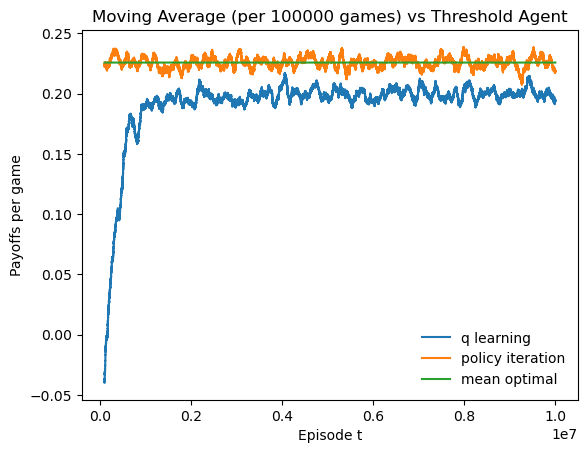
\includegraphics[width=0.33\textwidth, angle =0, trim = 0mm 0mm 0mm 0mm,clip=true]{figures/moving_averages_threshold}}
	\subfloat[]{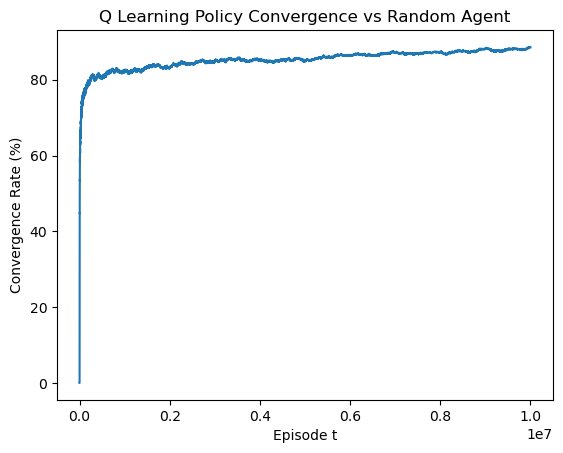
\includegraphics[width=0.33\textwidth, angle =0, trim = 0mm 0mm 0mm 0mm,clip=true]{figures/convergence_rate}}
\caption{Results of the first training instances per opponent and hyperparameter value set. (a)-(b) Moving average of payoffs (per $10^5$ games) against Random and Threshold agents respectively. (c) Similarity of policy returned by Q-learning compared to Policy Iteration, as a convergence rate indicator. Tables \ref{table:random-results}-\ref{table:threshold-results} show the hyperparameter values used for each legend entry.
}
\label{fig:1}
\end{figure}

\subsubsection{Random opponent}

Seeing the test results of all different agents against a Random opponent (Table \ref{table:random-results}), we can clearly confirm the theoretical ability of Q-learning to converge (in the limit) to the optimal policy. More specifically, allowing more exploration with $\epsilon$-greedy (with higher initial value and slower decay rate), Q-learning achieved almost the same reward distributions as with Policy Iteration. On the contrary, slowing down the decay of learning rate $\alpha$, without a similar decrease for $\epsilon$, significantly deteriorated performance. This effect of high learning rates is well-known, since they tend to introduce instability, preventing rapid convergence to the optimal solutions.

One way to analyze the speed of this algorithm's convergence is to inspect the flattening of the average rewards curve while training (Figure \ref{fig:1}(a)). Apart from the unstable case of large learning rate values, we can see that the linear part of the curve ends pretty fast, even before reaching $5\cdot10^5$ game episodes. 

Since the effect of $\epsilon$-greedy exploration does not allow us to understand whether these training sessions converge to optimal or suboptimal policies, I also introduced another way of convergence rate analysis by directly comparing the similarity of the Q-learning policy with the optimal policy returned by Policy Iteration (Figure \ref{fig:1}(c)). The superior hyperparameter configurations of the test results also become obvious here, since they are the ones reaching the highest attained similarity levels ($>$95\%), while speed of convergence is also reconfirmed (90\% reached with less than $5\cdot10^5$ games). Note that a few differences in policies obtained by Q-learning may be expected, since there are states where different actions are simultaneously optimal.

\subsubsection{Threshold opponent}

+++ TODO

%\begin{itemize}
%\item Implementation
%\item Analysis of hyperparameter tuning 
%\item Average Results
%\item Convergence analysis
%\end{itemize}

\section{Conclusion}

This course project was an excellent introduction to the basic principles of Reinforcement Learning and problem formulation. Designing and programming the environment for a novel poker variant I had the opportunity to hone my skills in modeling state-action space abstractions suitable for learning algorithms to utilize. Furthermore, implementing both Policy Iteration and Q-learning algorithms allowed me to understand the intricacies of their theory in action. Having full knowledge of the opposing agent's playstyle, Policy Iteration quickly solved the problem optimally. Even without this knowledge though, Q-learning proved capable of achieving similar performances after a relatively short number of training episodes. However, when the state-space differed due to the unknown nature of the opponent, Q-learning was not able to achieve the reward levels achieved by Policy Iteration, hinting that some kind of modeling assumptions and approximations may still be required in such cases.

\clearpage

\section*{Appendix}

\begin{table}[htpb]
\centering
\resizebox{0.9\linewidth}{!}{%
\begin{tabular}{ |p{0.2\linewidth}|p{0.2\linewidth}|p{0.3\linewidth}|p{0.3\linewidth}| }
\hline
Feature & Value Range & Necessity & Minimization\\
\hline
\hline
position & `first', `second' & Playing first or second has a direct consequence on the list of legal actions, and in case of Threshold agent, on the inferred hand range. & Unlike real poker, the simplification of retaining the same position for round 2 (flop) reduces number of possible transitions. \\
\hline
chips placed so far by currently acting player & `0.5', `1.5', `2.5', `3.5' & Knowing how many chips are already committed by player directly contributes to eventual rewards/losses. & `4.5' is omitted since it is only encountered in game terminal states\\
\hline
difference in chips of opposing player & `-1', `0', `1' & Knowing how many chips are already committed by opposing player efficiently merges information about eventual rewards/losses and current player's legal actions. & Since this is a limit hold'em game, this enumeration is smaller than using `0.5', `1.5', `2.5', `3.5', `4.5' directly.\\
\hline
rank of card in hand of currently acting player & `T', `J', `Q', `K', `A' & Strength of the card directly affects the player's chances of winning if no player folds until the end of round 2 & Suit does not matter at all in the simplified winning conditions of this game version, therefore it can be completely omitted from state-space representation.\\
\hline
rank of remaining possible opposing player cards in hand in alphabetical order & `none' if not revealed yet, else all 10 combinations (e.g. `AK', `AJ', `JK' etc.) & Strength of the card directly affects the player's chances of winning if no player folds until the end of round 2 & Suit does not matter at all in the simplified winning conditions of this game version, therefore it can be completely omitted from state-space representation. Furthermore, the order of public cards does not matter in this variant, hence the alphabetical order offers a consistent way of reducing the number of states.\\
\hline
rank of remaining possible opposing player cards in hand in alphabetical order & Based on Table \ref{table:threshold-actions}: `AJKQT' (no information), `JQT', all 10 combinations of public hands, and all ranks (when the opposing hand's rank is surely known) & Needed only for Threshold agent, the strength of the opposing hand directly affects the player's chances of winning if no player folds until the end of round 2, and it also determines the probability of the Threshold agent's next action & When the opposing agent is not known to be the Threshold agent, only `AJKQT' is used. See above too.\\
\hline
\end{tabular}
}
\caption{Simplified poker state-space representation utilized by Policy Iteration and Q-learning algorithms.}
\label{table:state-space}
\end{table}

\begin{table}[htpb]
\centering
\resizebox{0.9\linewidth}{!}{%
\begin{tabular}{ |c|c|c|c| }
\hline
agent & hyperparameters &average reward & standard deviation\\
\hline
\hline
Policy Iteration & $\gamma=1$, $\delta=10^{-10}$ & 0.8761 & 2.127\\
\hline
Threshold & - & 0.3094 & 1.643\\
\hline
q\_base & $\epsilon_0=1$, $\alpha_0=1$, $\epsilon_d=-1/8$, $\alpha_d=-1/4$ & 0.8670 & 2.121\\
\hline
q\_slower\_alpha & $\epsilon_0=1$, $\alpha_0=1$, $\epsilon_d=-1/4$, $\alpha_d=-1/8$ & 0.4862 & 1.655\\
\hline
q\_lower\_alpha & $\epsilon_0=1$, $\alpha_0=0.1$, $\epsilon_d=-1/8$, $\alpha_d=-1/4$ & 0.8329 & 2.103\\
\hline
q\_slower\_epsilon & $\epsilon_0=1$, $\alpha_0=1$, $\epsilon_d=-1/16$, $\alpha_d=-1/4$ & 0.8733 & 2.128\\
\hline
q\_slower\_decay & $\epsilon_0=1$, $\alpha_0=0.1$, $\epsilon_d=-1/16$, $\alpha_d=-1/8$ & 0.8739 & 2.128\\
\hline
\end{tabular}
}
\caption{Testing performance of various agents against Random agent. All experiments consisted of a total number of $5\cdot10^6$ games.}
\label{table:random-results}
\end{table}

\begin{table}[htpb]
\centering
\resizebox{0.9\linewidth}{!}{%
\begin{tabular}{ |c|c|c|c| }
\hline
agent & hyperparameters &average reward & standard deviation\\
\hline
\hline
Policy Iteration & $\gamma=1$, $\delta=10^{-10}$ & 0.2252 & 1.467\\
\hline
q\_base & $\epsilon_0=1$, $\alpha_0=0.1$, $\epsilon_d=-1/8$, $\alpha_d=-1/4$ & 0.1623 & 1.246\\
\hline
q\_slower\_alpha & $\epsilon_0=1$, $\alpha_0=0.1$, $\epsilon_d=-1/8$, $\alpha_d=-1/8$ & 0.1491 & 1.149\\
\hline
q\_bigger\_alpha & $\epsilon_0=1$, $\alpha_0=1$, $\epsilon_d=-1/8$, $\alpha_d=-1/4$ & 0.1460 & 1.100\\
\hline
q\_slower\_epsilon & $\epsilon_0=1$, $\alpha_0=0.1$, $\epsilon_d=-1/16$, $\alpha_d=-1/4$ & 0.1549 & 1.351\\
\hline
q\_slower\_decay & $\epsilon_0=1$, $\alpha_0=0.1$, $\epsilon_d=-1/16$, $\alpha_d=-1/8$ & 0.1553 & 1.212\\
\hline
\end{tabular}
}
\caption{Testing performance of various agents against Threshold agent. All experiments consisted of a total number of $5\cdot10^6$ games.}
\label{table:threshold-results}
\end{table}





%--------------------------------------------------

%In this report I analyze the performance of Multiplicative Weights (MW) algorithms in ``Experts'' and ``Adversarial Bandits'' environments. As an example, a normalized dataset of real traffic loads for $k=30$ servers and a duration of $T=7000$ rounds was provided. The goal of the algorithms is to predict and pick the least loaded server at each time round. 
%
%\subsection*{Part I}
%
%\subsubsection*{1.1 MW and hyperparameter values}
%
%The implementation between the MW variants has a shared base structure, varying only in the amount of information acquired per round (Experts vs Bandits environment) and how this assumption is then applied to updating the weights for the selection process.
%
%More specifically, for the Experts environment, the learning algorithm acquires the normalized load (loss) of every server at each round $t$. Following our lecture notes \footnote{lecture19, Expert\_Adv\_Bandit\_Lecture}, I implemented the updating algorithm and set the hyperparameter $\eta=\sqrt{\frac{\ln{k}}{{T}}}$, which theoretically gives sublinear regret over the horizon ($O(\sqrt{T\ln k})$).
%
%In regards to the Bandits' environment, the algorithm only gets the load of the selected server at round $t$. Following the respective analysis in our lecture notes \footnote{lecture20, Expert\_Adv\_Bandit\_Lecture}, we now have to set an exploration hyperparameter $\epsilon$, which is a balancing factor between exploration and exploitation. In this report, I present results for two values: 1) $\eta=\epsilon=\sqrt{\frac{\ln{k}}{{T}}}$ (titled ``explore less''), and 2) $\eta=\epsilon=\sqrt[\leftroot{-2}\uproot{2}3]{\frac{n\ln{k}}{{T}}}$ (titled ``explore more'').
%
%\subsubsection*{1.2 Experts vs Bandits}
%
%\figref{fig:1} shows the results of one realization per algorithm for $T=1000$ (Subfigures a-c) and $T=7000$ (Subfigures d-f). Subfigures (a,d) show the total loss accumulated at each round $t$, (b,e) show the cumulative regret at each $t$, and (c,f) show the average regret over $t$. For the calculation of regrets, I used the loss provided by picking the best server over the horizon (server i = 12 in both cases).
%
%Expectedly due to full observability, the Experts setup has the superior performance over both small and large horizon $T$. At $T=7000$ it seems it has reached a point where the cumulative regret no longer significantly increases. On the contrary, the adversarial bandits setup accumulates more regret over time, and still shows accumulation at the end of the horizon. Nevertheless, the curve for the algorithm with less exploration has a shape similar to that of Experts, which is indicative of the similar regret bound of $O(\sqrt{kT\ln k})$ (the extra $k$ term being the penalty of partial observability).
%
%\subsubsection*{1.3 Exploration with Bandits}
%
%Interesting observations are made by inspecting the behavior of the ``explore more'' adversarial bandits case. Since $\eta$ is also higher for this implementation, it is obvious that bad servers are more severely penalized, resulting in better server choices in the short term. However, since the exploration probability is higher too, the ``explore more'' Bandits variant eventually accumulates more regret than both the Experts and the ``explore less'' variants. While the ``explore more'' variant seems at a long-term disadvantage, we should factor in the purpose of this algorithm: high value of $\epsilon$ may lead to more bad options, but the reasoning behind it is that under an adversarial setting, these so-far bad options may turn out to be good. Therefore, we should expect this algorithm to adapt faster to sudden changes of the best server over time.
%
%\begin{figure}[htpb]
%\renewcommand*\thesubfigure{\alph{subfigure}}
%\centering
%	\subfloat[]{\includegraphics[width=0.33\textwidth, angle =0, trim = 0mm 0mm 0mm 0mm,clip=true]{figures/total_loss_30_1000}}
%	\subfloat[]{\includegraphics[width=0.33\textwidth, angle =0, trim = 0mm 0mm 0mm 0mm,clip=true]{figures/total_regret_30_1000}}
%	\subfloat[]{\includegraphics[width=0.33\textwidth, angle =0, trim = 0mm 0mm 0mm 0mm,clip=true]{figures/average_regret_30_1000}}\\
%	\subfloat[]{\includegraphics[width=0.33\textwidth, angle =0, trim = 0mm 0mm 0mm 0mm,clip=true]{figures/total_loss_30_7000}}
%	\subfloat[]{\includegraphics[width=0.33\textwidth, angle =0, trim = 0mm 0mm 0mm 0mm,clip=true]{figures/total_regret_30_7000}}
%	\subfloat[]{\includegraphics[width=0.33\textwidth, angle =0, trim = 0mm 0mm 0mm 0mm,clip=true]{figures/average_regret_30_7000}}
%\caption{Performance of Multiplicative Weights (MW) and Upper Confidence Bound (UCB) algorithms on predicting the least loaded server out of $k=30$ at every time round $t$. 
%%Results of three MW algorithms are presented; one implementation assuming full observability of all servers' loads at each round $t$ (called ``Experts''), and two assuming observability only of the selected server (called ``Bandits''). For Bandits variants, effect of exploration parameter $\gamma$ is illustrated. Subfigures (a-c) and (c-f) show a realization for horizon $T=1000$ and $7000$ respectively. In both cases, the server $i=12$ was the least loaded for the respective duration.
%}
%\label{fig:1}
%\end{figure}
%
%\subsection*{Part II}
%
%\subsubsection*{2.1 Modifications to UCB for losses instead of rewards}
%
%In this part, I adapted the UCB algorithm of programming assignment 1 to this assignment's problem. Since in assignment 1 the algorithm was maximizing rewards instead of minimizing losses, I simply negated the provided dataset values. As a result, no modification was required for the algorithm internally, and the algorithm simply maximized negative losses, which is equivalent to minimizing the losses (as positive values).
%
%\subsubsection*{2.2 UCB vs Bandits}
%
%As expected for adversarial bandits, UCB consistently exhibits the worst performance, which agrees with the theoretical linear regret bound. Nevertheless, for this particular dataset, it is clear that even UCB shows a curve saturation over time. If a particular server is consistently and/or significantly better than the others over the horizon, which seems to be the case for server $i=12$, then the environment is practically less ``adversarial'' and more ``stochastic'' in nature, and UCB will predictably perform better over time.